\section{How to read every graph}
\label{ch:figures}

Every figure in the ICLR draft and the technical report, with the same four
questions asked of each: what is on the axes, what one mark is, what to look
for, and the sentence you should be able to say about it. Figures are shown
small here; the full-size versions are in the documents. Read a graph in this
order: axes first, then one mark, then the pattern, then the caption's claim,
and check that the pattern supports the claim.

\subsection{The two figures in the ICLR paper}

\begin{figure}[h]\centering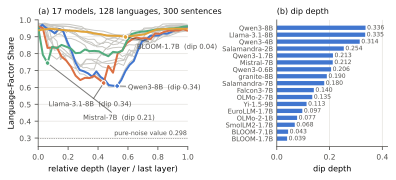
\includegraphics[width=0.95\linewidth]{figs/report/paper_fig1.png}
\caption{Paper Figure 1. (a) LFS against relative depth for 17 models; (b) dip depth per model.}\label{fig:g-p1}\end{figure}

\paragraph{Paper Figure 1(a).} Horizontal axis: relative depth, layer index
divided by the last layer, so that a 25-layer model and a 49-layer model can
share one axis (0 is the embedding output, 1 is the last block). Vertical
axis: LFS at that layer, computed on the 128 by 300 grid. One line is one
model; 17 lines, four named. The dashed horizontal line at $0.298$ is the
pure-noise value $(L-1)/(L+N-2)$ for this grid size: a grid of random noise
with no language or content structure would sit there. What to look for:
every line starts high, near $0.93$ to $0.98$, drops to a minimum somewhere
in the interior, and rises again toward the output; the depth of the drop
differs enormously (Qwen3-8B and Llama-3.1-8B fall to about $0.61$, BLOOM
barely moves); every line stays above the noise value at every layer, so the
language component is real everywhere, and the question is only how large it
is relative to content. Sentence to say: ``Representations start
language-organized, become most meaning-weighted in the middle, and
re-separate by language toward the output, in every model, by amounts that
vary nine-fold.''

\paragraph{Paper Figure 1(b).} Horizontal bars, one per model, sorted:
dip depth, which is the first-layer LFS minus the minimum LFS. Read it as a
ranking with the caveat from the bootstrap: neighbouring bars within about
$0.02$ are not distinguishable, and Mistral-7B and Salamandra-2B have wider
intervals because their minimum sits at layer 2 or 6.

\begin{figure}[h]\centering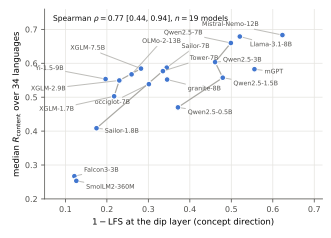
\includegraphics[width=0.62\linewidth]{figs/report/paper_fig2.png}
\caption{Paper Figure 2. The model-level content-transfer result.}\label{fig:g-p2}\end{figure}

\paragraph{Paper Figure 2.} Horizontal axis: $1 - \mathrm{LFS}$ at the dip
layer, the sentence-component share $1-$LFS-VC, so models further right are more
meaning-weighted at their dip. Vertical axis: the model's median
$R_{\mathrm{content}}$ over 34 languages, which is how much a foreign-language
context sentence helps the model predict an English continuation when the
context is the matched translation rather than a mismatched one, normalized by
the English-context benefit. One dot is one of the 19 frozen models; gray
connectors join sizes within a family. What to look for: the cloud rises to
the right, Spearman $0.77$ with model-bootstrap interval $[0.44, 0.94]$;
SmolLM2-360M and Falcon3-3B sit bottom-left, Mistral-Nemo and Llama-3.1-8B
top-right; within a family the connector also rises. Sentence to say: ``Models
whose middle layers weight meaning more make more use of foreign-language
context, and the association holds at the level of whole models, not only
pooled rows.'' Caveat: 19 dots is a small sample; the interval is wide and the
paper says so.

\subsection{The technical report, in order}

\begin{figure}[h]\centering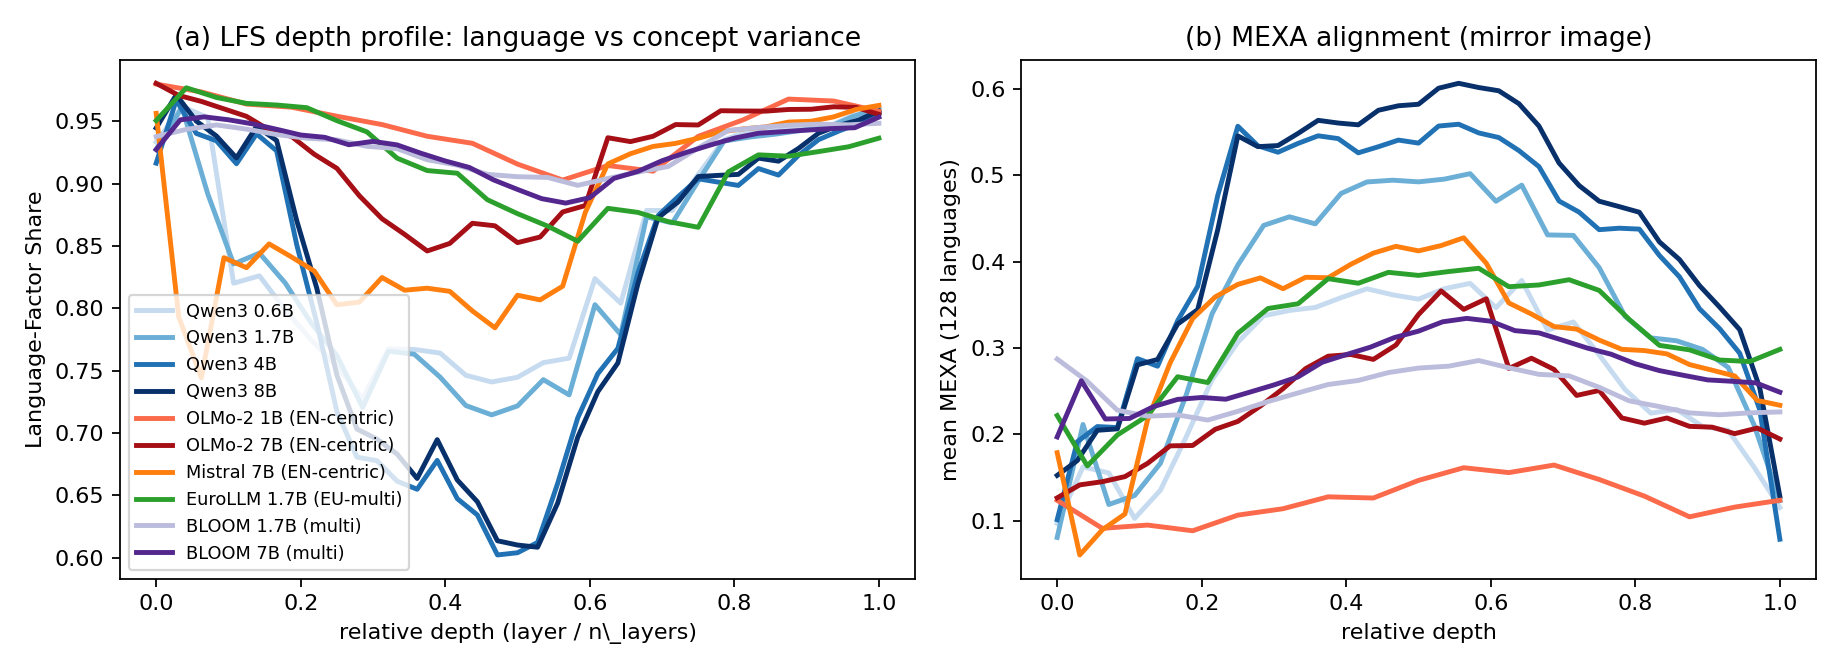
\includegraphics[width=0.95\linewidth]{figs/report/fig1_lfs_depth_profile.png}
\caption{Report Figure 1. (a) LFS by depth, development grid; (b) mean MEXA by depth.}\label{fig:g-r1}\end{figure}

\paragraph{Report Figure 1.} Same axes as paper Figure 1(a), for the ten
development models, coloured by family (Qwen3 blues, OLMo-2 reds, Mistral
orange, EuroLLM green, BLOOM purples). Panel (b) plots mean MEXA, the
published retrieval measure, on the same depth axis. What to look for: (b)
is roughly the mirror image of (a). Where the language share is lowest,
retrieval of the matched translation is easiest. Sentence: ``Two different
instruments agree on where the middle is.'' Do not read (b) as a competition;
it is shown so a reader who knows MEXA can place LFS.

\begin{figure}[h]\centering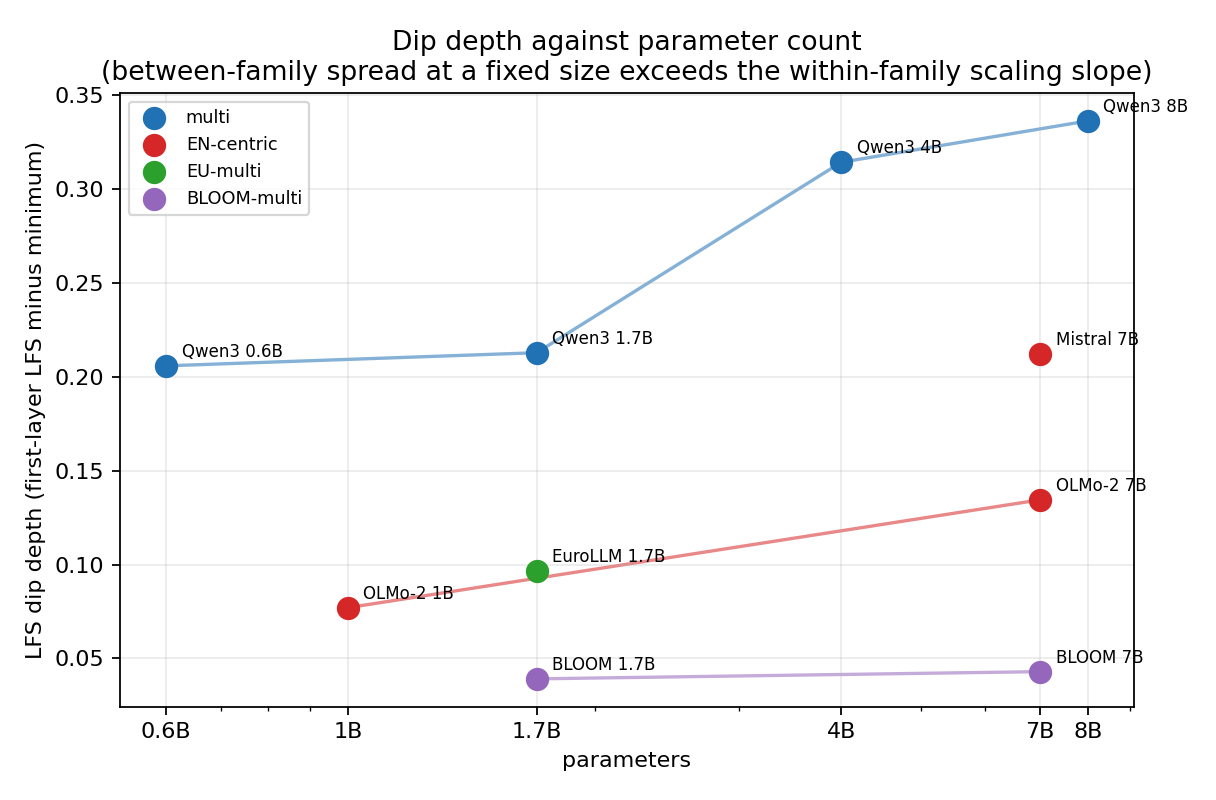
\includegraphics[width=0.66\linewidth]{figs/report/fig7_mix_vs_scale.png}
\caption{Report Figure 2. Dip depth against parameter count.}\label{fig:g-r7}\end{figure}

\paragraph{Report Figure 2 (dip depth against parameters).} Horizontal axis:
parameter count, on a compressed scale. Vertical axis: dip depth. One dot is
one model, coloured by training-mix class; lines join sizes within a family.
What to look for: within a family the line slopes up (scale deepens the dip),
but at a fixed size the vertical spread across families is far larger than
any slope. Near 7B the dots run from BLOOM at $0.04$ through OLMo-2 at $0.13$
and Mistral at $0.21$ to Qwen3-8B at $0.34$. Sentence: ``How a model was
trained moves the dip more than how big it is.'' Caveat: dots within about
$0.02$ of each other, such as Qwen3-1.7B at $0.213$ and Mistral-7B at
$0.212$, are not distinguishable once the bootstrap intervals are attached.

\begin{figure}[h]\centering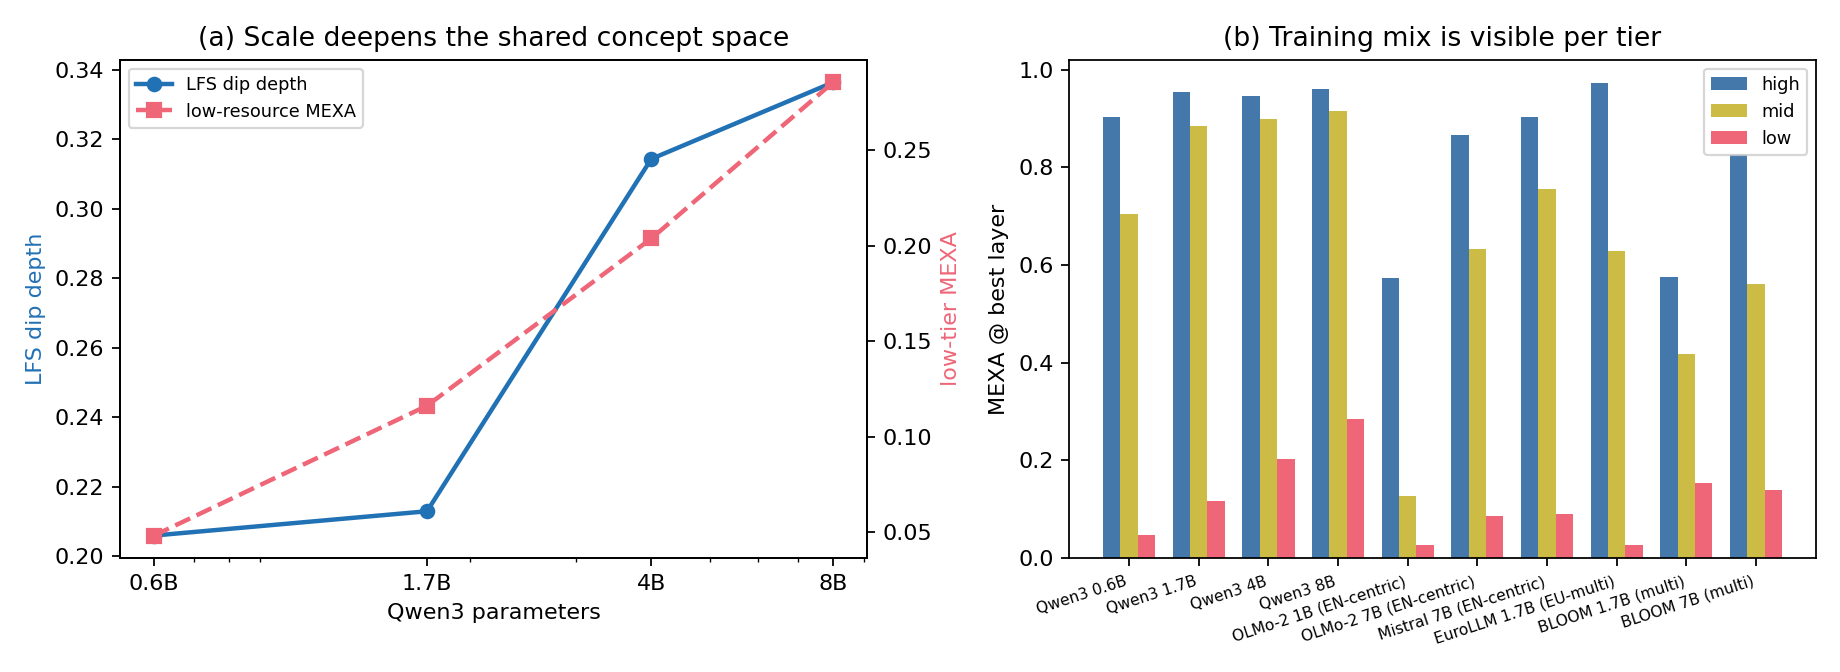
\includegraphics[width=0.95\linewidth]{figs/report/fig2_scaling_tiers.png}
\caption{Report Figure 3. (a) Qwen3 series with two vertical axes; (b) MEXA by resource tier.}\label{fig:g-r2}\end{figure}

\paragraph{Report Figure 3.} Panel (a) has two vertical axes: dip depth on
the left (blue, solid) and low-resource-tier MEXA on the right (red, dashed),
both against Qwen3 size. Read each line against its own axis only; the
crossing point means nothing, because the two scales were chosen
independently. What it shows: both rise with scale within Qwen3. Panel (b):
for each model, three bars, MEXA at the best layer averaged over high-, mid-,
and low-resource languages. What to look for: the low-resource bar is near
the floor for OLMo-2, EuroLLM, and BLOOM, and rises with scale only for
Qwen3. Sentence: ``The training mix is visible tier by tier.'' Caveat: this
is a four-point trend for one family; the paper does not generalize it.

\begin{figure}[h]\centering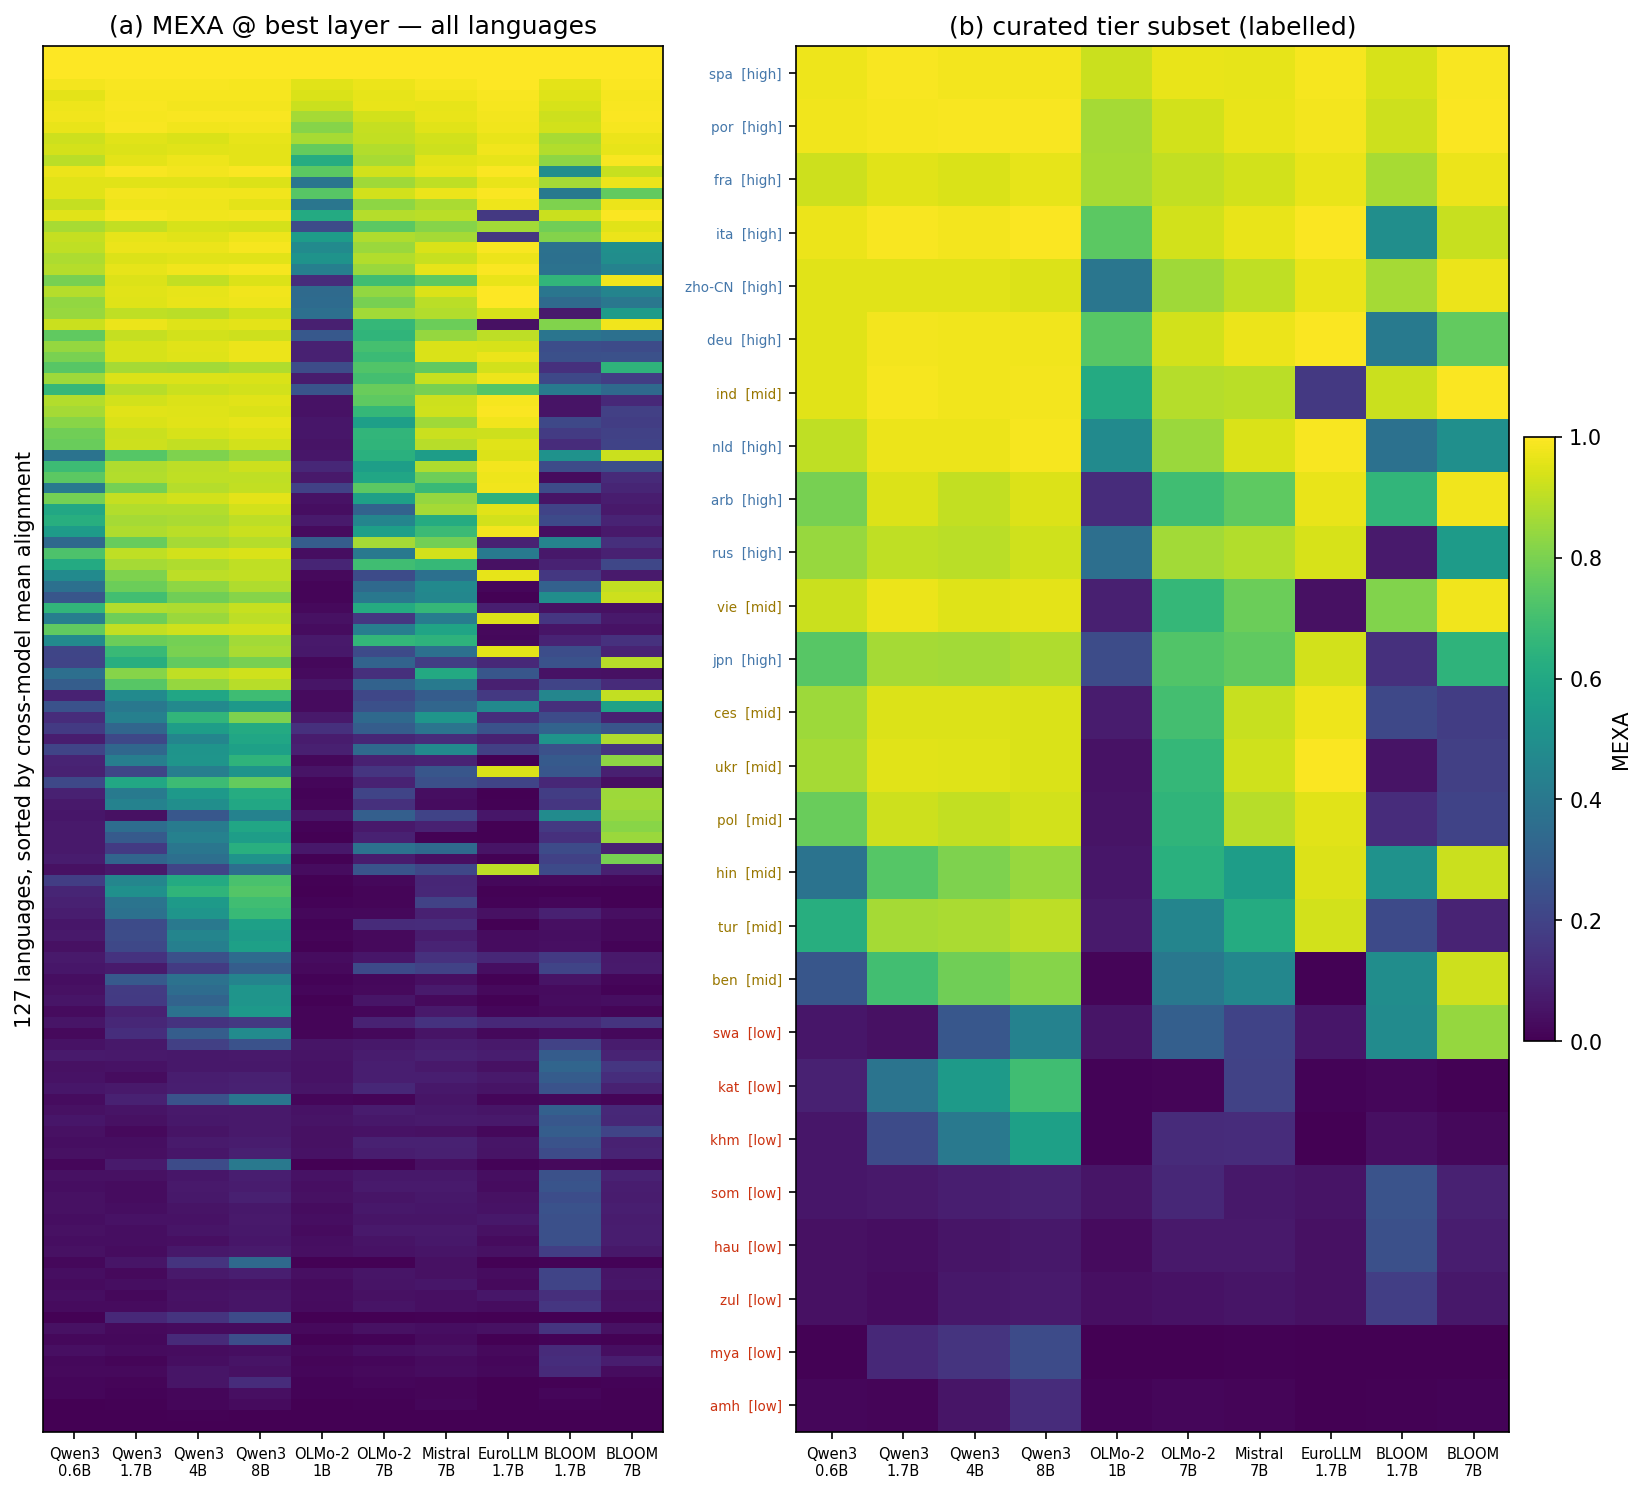
\includegraphics[width=0.95\linewidth]{figs/report/fig6_heatmap.png}
\caption{Report Figure 4. MEXA at the best layer, languages by models.}\label{fig:g-r6}\end{figure}

\paragraph{Report Figure 4 (heatmap).} Rows are 127 languages sorted by their
mean alignment across models; columns are the ten development models; colour
is MEXA at the best layer, dark for 0 and yellow for 1. Panel (b) is a 26
language subset with labels and resource tiers. How to read: run your eye down
a column to see a model's pattern (Qwen3 columns bright far down, OLMo-2
dark outside the top band, EuroLLM bright exactly on its European block);
run across a row to see how a language fares everywhere. The bottom rows are
dark for every model. Sentence: ``The lowest-resource languages are unaligned
in every model; the models differ in how far down the list alignment
reaches.'' This is a reference measure, not an LFS result.

\begin{figure}[h]\centering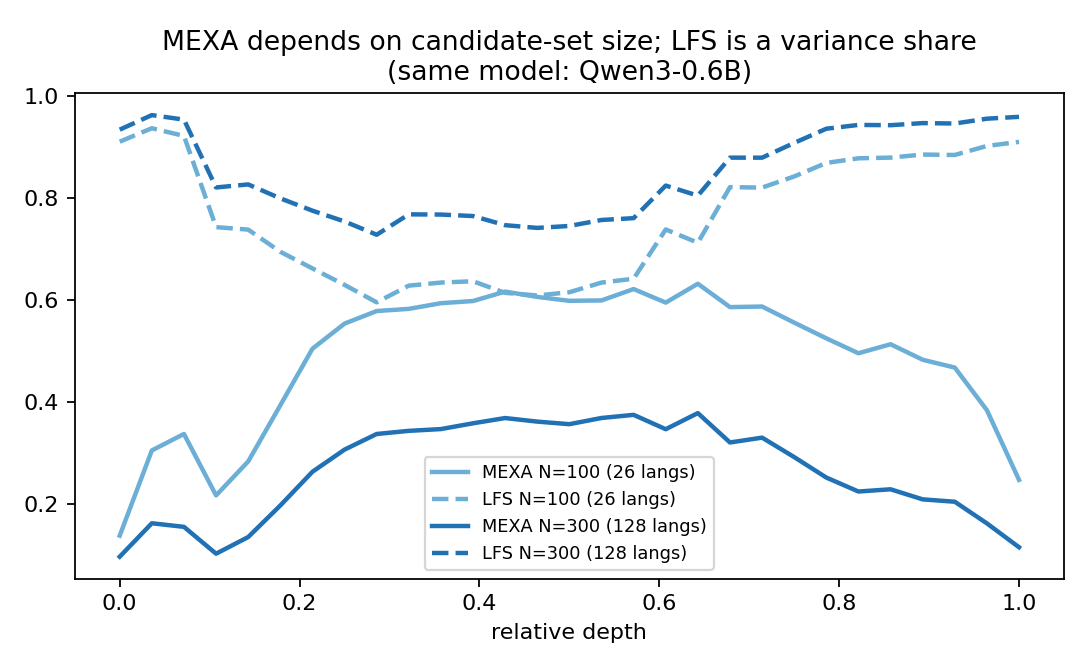
\includegraphics[width=0.7\linewidth]{figs/report/fig5_n_sensitivity.png}
\caption{Report Figure 5. Evaluation-size dependence.}\label{fig:g-r5}\end{figure}

\paragraph{Report Figure 5.} Depth on the horizontal axis; four curves for
one model, Qwen3-0.6B: MEXA (solid) and LFS (dashed) each computed with 100
sentences and 26 languages, and with 300 sentences and 128 languages. What to
look for: the two MEXA curves are far apart (the peak falls from about $0.63$
to $0.38$) because retrieval gets harder with more decoys, while the two LFS
curves nearly coincide. Sentence: ``A retrieval score depends on how many
candidates you gave it; a variance share does not.'' The report quantifies
the small residual dependence of LFS elsewhere rather than claiming exact
invariance.

\begin{figure}[h]\centering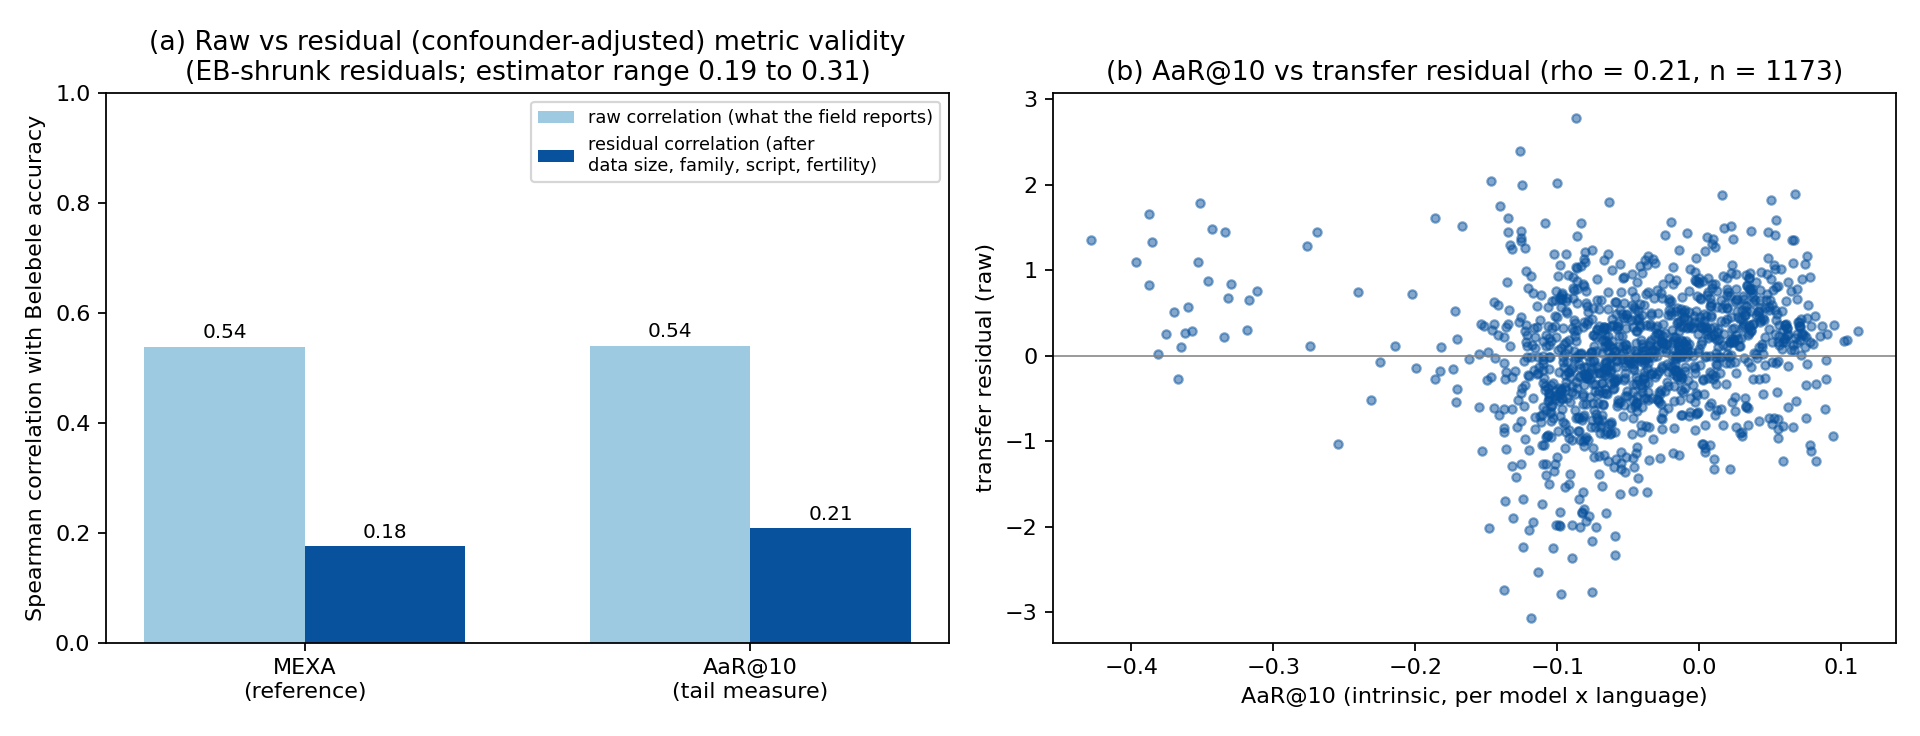
\includegraphics[width=0.95\linewidth]{figs/report/fig8_deflation.png}
\caption{Report Figure 6. Raw and confounder-adjusted validity against benchmark accuracy.}\label{fig:g-r8}\end{figure}

\paragraph{Report Figure 6 (confounder adjustment).} Panel (a): for the tail measure
AaR@10 and, for reference, MEXA, two bars each: the raw Spearman correlation
with Belebele accuracy across (model, language) rows, and the residual
correlation after regressing out training-data size, language family, script,
and tokenizer fertility from both variables. What to look for: both fall from
about $0.5$ to about $0.2$. Panel (b): the residual scatter for AaR@10, 690
rows, a weak positive cloud. Sentence: ``About half of the raw correlation is
data exposure; what survives is the metric's own information.'' The two
measures are not ranked against each other.

\begin{figure}[h]\centering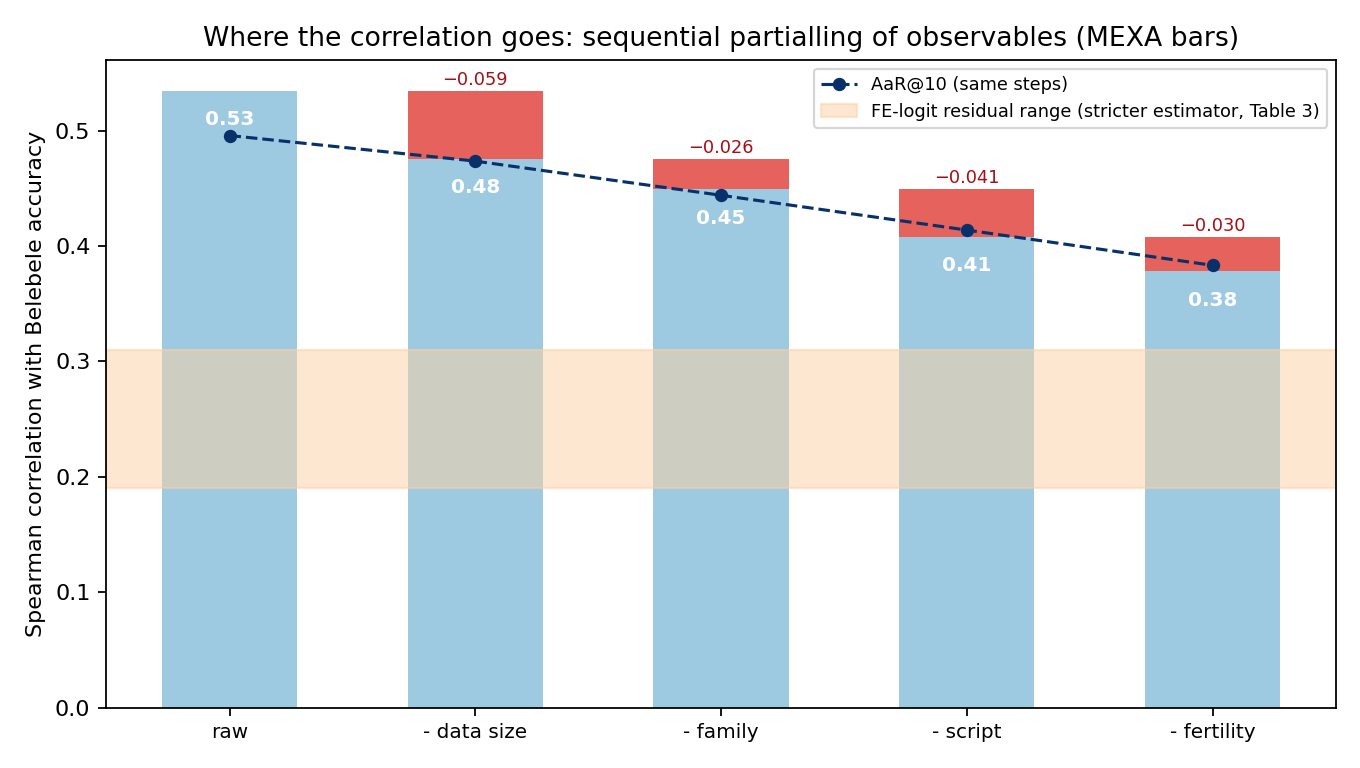
\includegraphics[width=0.78\linewidth]{figs/report/fig11_waterfall.png}
\caption{Report Figure 7. Sequential partialling of observables.}\label{fig:g-r11}\end{figure}

\paragraph{Report Figure 7 (sequential partialling).} Bars from left to right: the raw
correlation, then the correlation after removing data size, then also family,
then also script, then also fertility. The red cap on each bar is the amount
the last control removed. The dashed line repeats the steps for AaR@10. The
shaded band is the stricter fixed-effects estimate of the same quantity,
$0.19$ to $0.31$. What to look for: every control removes some, data size the
most; the sequence stops well above zero. Sentence: ``The correlation is
partly exposure, partly something the metric adds.'' Caveat stated in the
report: the order of controls affects the individual steps, not the endpoint.

\begin{figure}[h]\centering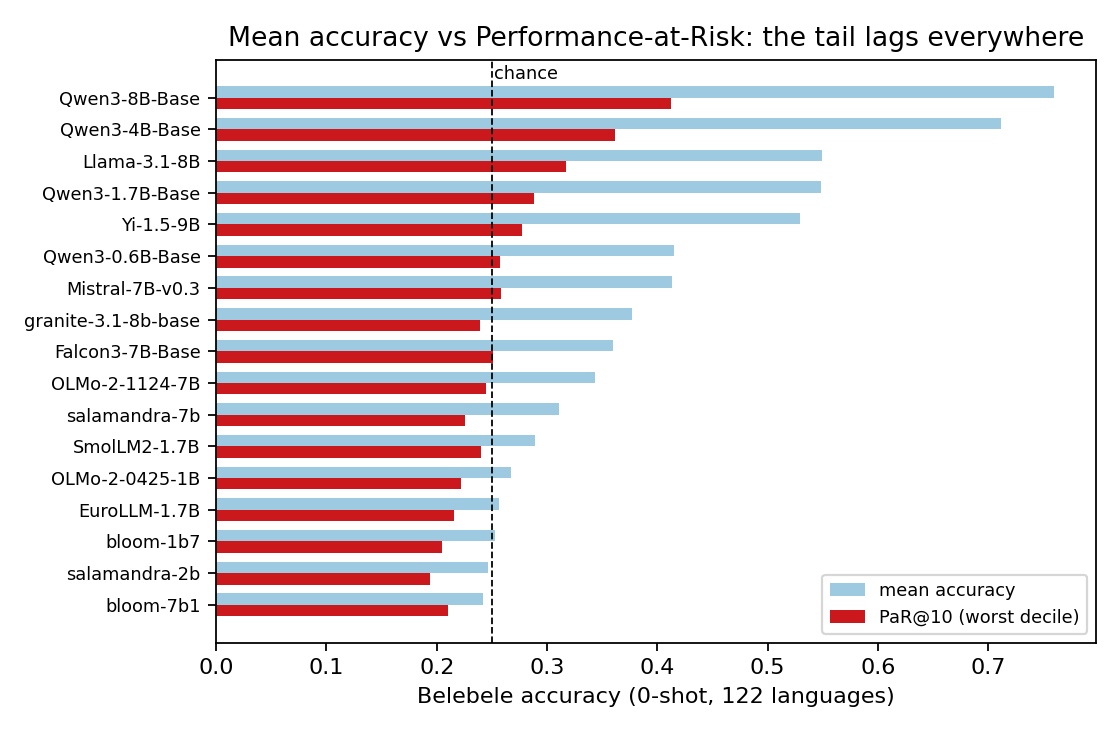
\includegraphics[width=0.7\linewidth]{figs/report/fig9_par.png}
\caption{Report Figure 8. Mean accuracy against worst-decile accuracy.}\label{fig:g-r9}\end{figure}

\paragraph{Report Figure 8 (Performance-at-Risk).} One row per model; light
bar is mean Belebele accuracy across 122 languages, red bar is PaR@10, the
mean accuracy over the worst ten percent of languages. The dashed line is
chance for a four-way benchmark, $0.25$. What to look for: the red bar lags the
light bar for every model, and for several models the red bar sits at chance
while the mean is comfortably above it. Sentence: ``The mean hides languages
on which the model is guessing.''

\begin{figure}[h]\centering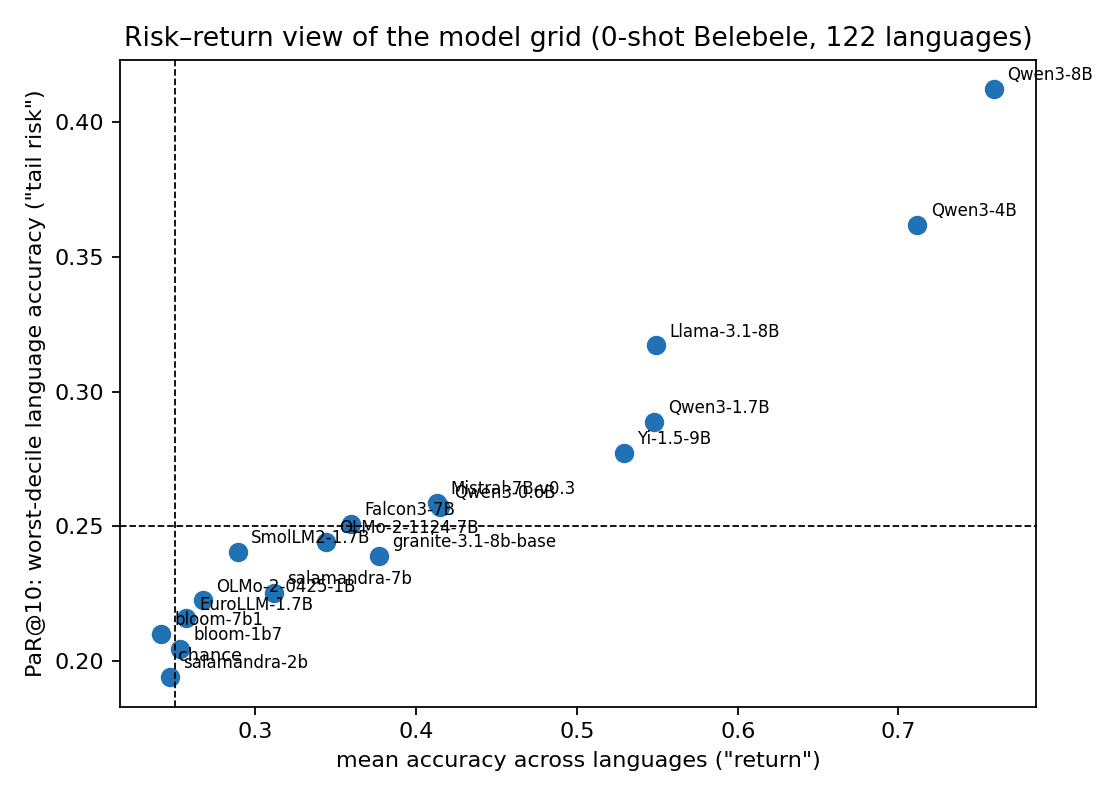
\includegraphics[width=0.66\linewidth]{figs/report/fig13_riskreturn.png}
\caption{Report Figure 9. Mean accuracy against tail accuracy, one dot per model.}\label{fig:g-r13}\end{figure}

\paragraph{Report Figure 9.} The same two numbers as Figure 8, now as a
scatter: mean accuracy horizontally, worst-decile accuracy vertically, dashed
chance lines on both. What to look for: Qwen3-8B is alone in the top right,
a cluster of models sits at the chance corner, and no model is high on one
axis and low on the other. Sentence: ``On this benchmark, serving the tail and
serving the average go together; nobody buys tail robustness by sacrificing
the mean.''

\begin{figure}[h]\centering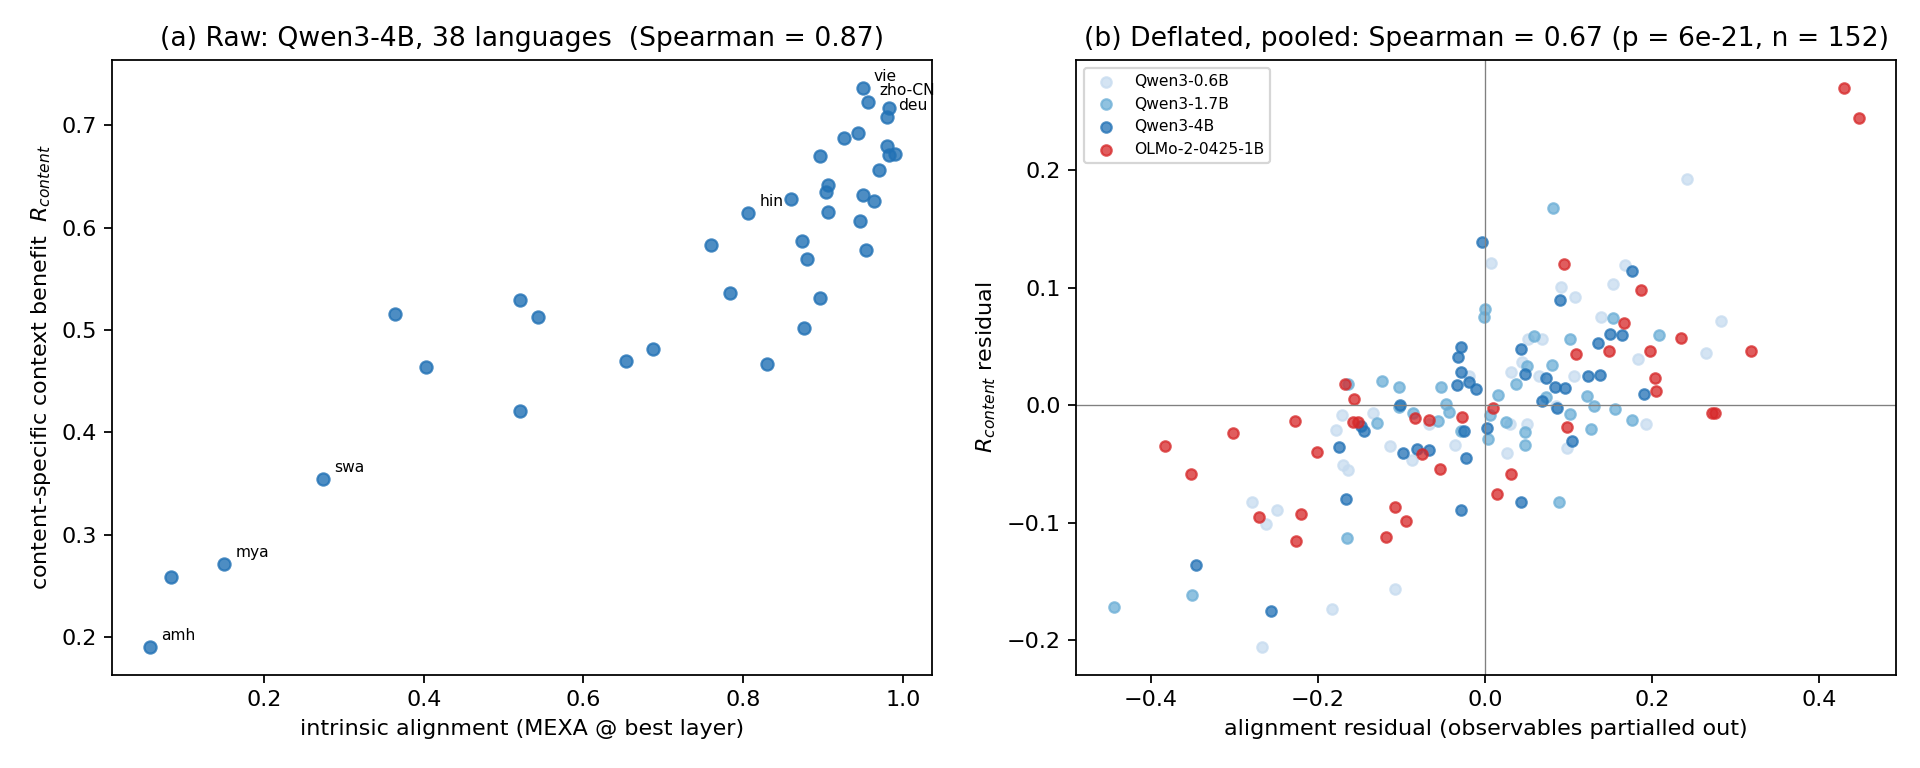
\includegraphics[width=0.95\linewidth]{figs/report/fig10_b2scatter.png}
\caption{Report Figure 10. Alignment against content-specific context benefit.}\label{fig:g-r10}\end{figure}

\paragraph{Report Figure 10.} Panel (a), one model (Qwen3-4B): each dot is a
language, horizontal is its alignment at the best layer, vertical is its
content-specific context benefit $R_{\mathrm{content}}$; Amharic, Burmese,
and Swahili sit bottom-left, German, Chinese, and Vietnamese top-right,
Spearman $0.87$. Panel (b): both axes replaced by their residuals after the
same four controls, pooled over four models and coloured by model; Spearman
$0.67$. What to look for: the cloud in (b) still rises. Sentence: ``The
relation between alignment and context use is not just resource level in
disguise.'' This is the four-model pilot; the 19-model version is paper
Figure 2.

\begin{figure}[h]\centering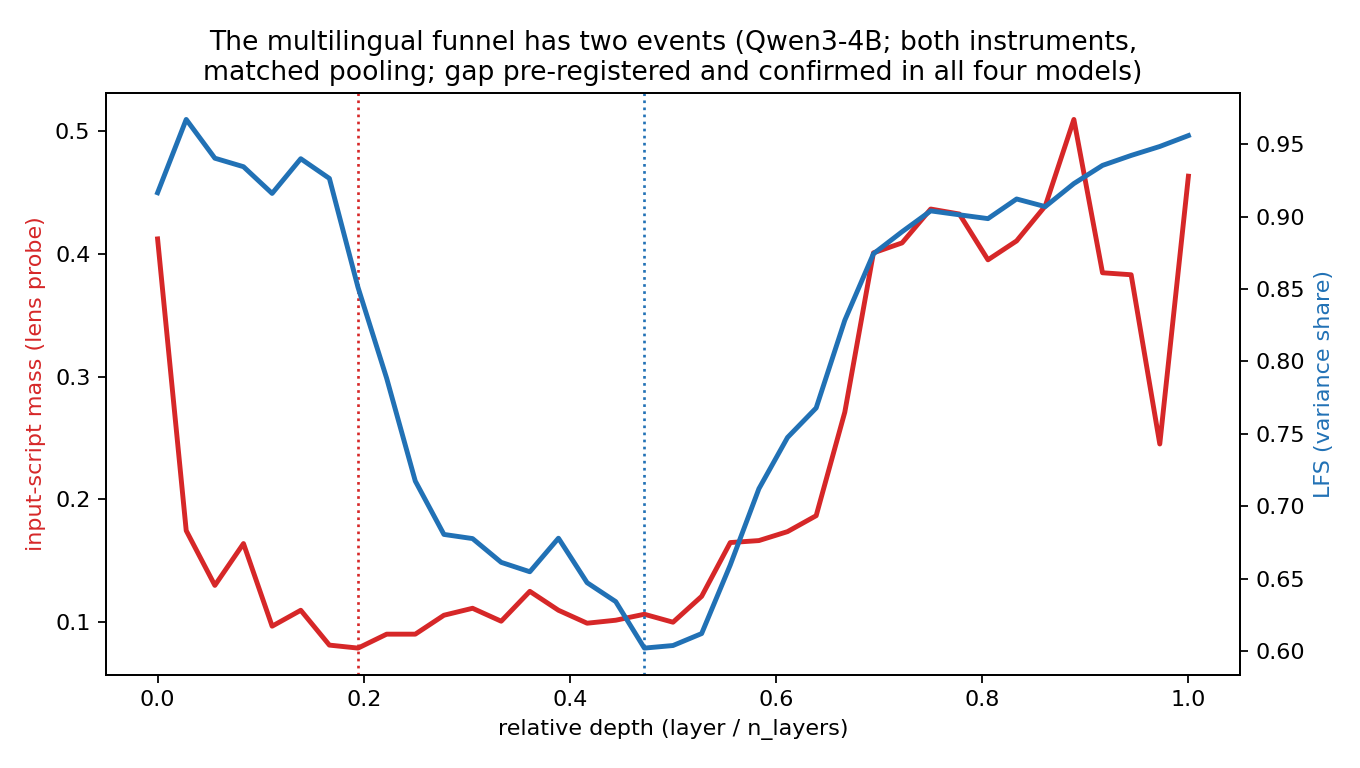
\includegraphics[width=0.78\linewidth]{figs/report/fig12_twoevents.png}
\caption{Report Figure 11. Two instruments on one depth axis.}\label{fig:g-r12}\end{figure}

\paragraph{Report Figure 11 (two events).} Two vertical axes again, so read
each curve against its own. Red, left axis: the share of probability mass the
logit lens puts on tokens in the input's script, which falls steeply by
relative depth $0.2$. Blue, right axis: LFS, which reaches its minimum near
$0.47$. Dotted verticals mark the two minima. Sentence: ``The surface script
is abandoned early; the language share of the variance converges later. They
are two events, not one.'' This is the report's evidence that a logit-lens
measure and a representation measure measure different things.

\begin{figure}[h]\centering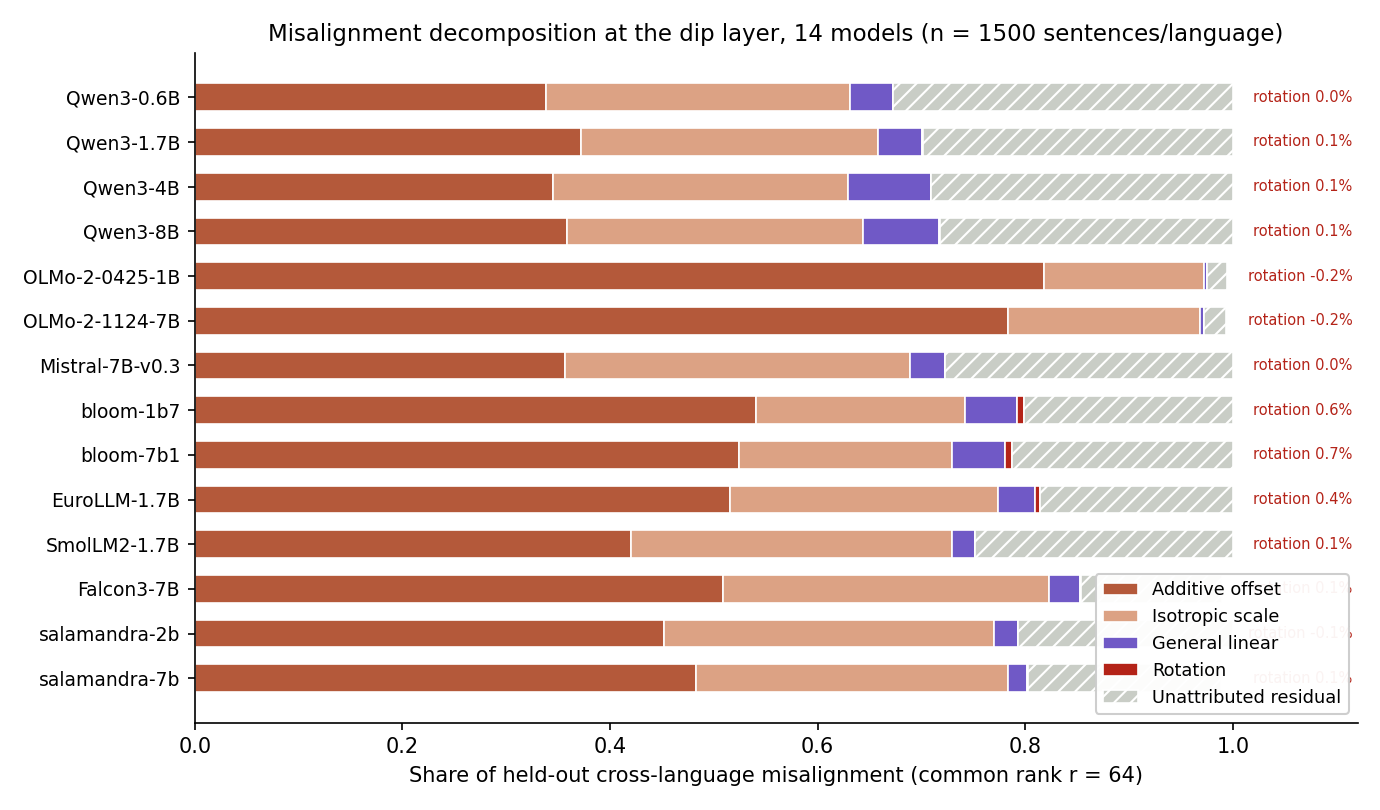
\includegraphics[width=0.95\linewidth]{figs/report/fig15_budget_composition.png}
\caption{Report Figure 12 and paper appendix figure. The misalignment decomposition.}\label{fig:g-r15}\end{figure}

\paragraph{Report Figure 12 (misalignment decomposition).} One stacked bar per
model, at the dip layer, on the 1,500-sentence 1,500-sentence data. The bar is the
held-out cross-language misalignment, split into what a nested sequence of maps
explains: an additive offset (dark), an isotropic scale (light), a general
linear map (purple), a rotation (red, barely visible), and an unattributed
remainder (hatched). Rotation shares are printed at the right. What to look
for: offset plus scale explain $0.63$ to $0.97$ of the misalignment in every
model, rotation never exceeds $0.7$ percent. Sentence: ``Languages differ
mostly by a shift and a stretch, which is exactly what an additive
decomposition can see; the construct boundary of LFS is empirically
harmless here.''

\begin{figure}[h]\centering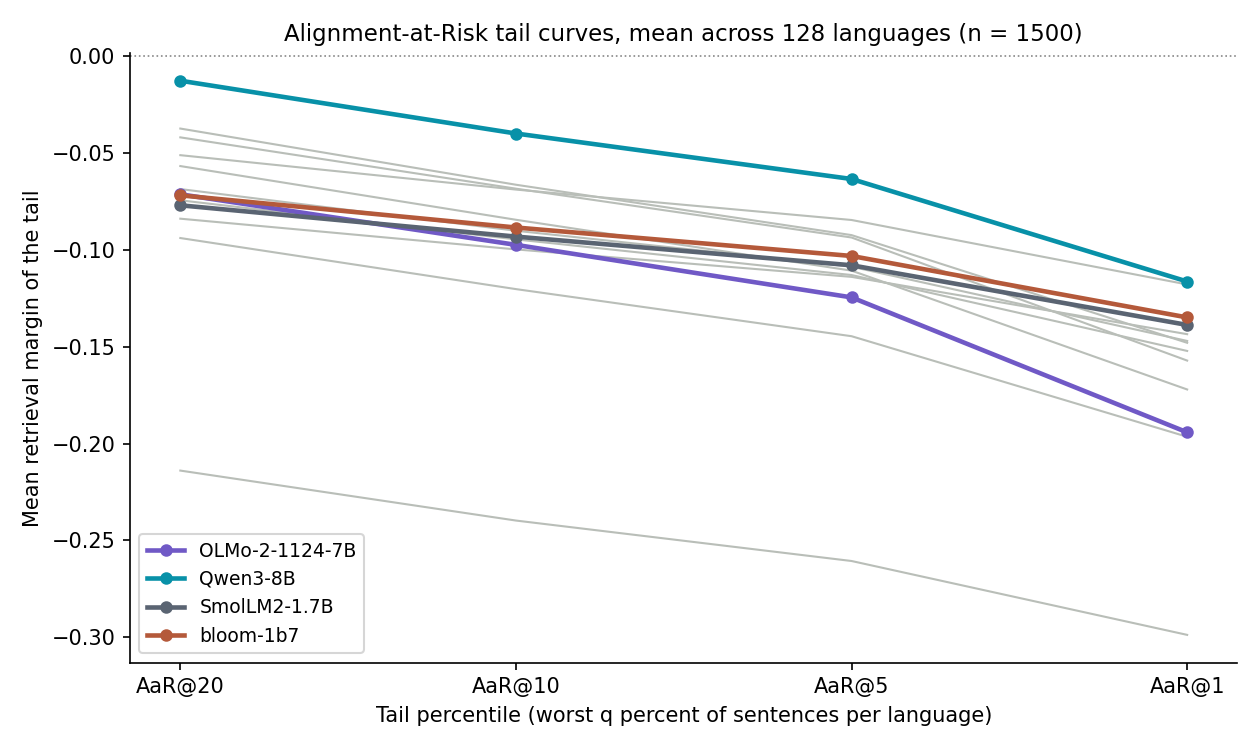
\includegraphics[width=0.78\linewidth]{figs/report/fig16_tail_curves.png}
\caption{Report Figure 13. Alignment-at-Risk tail curves.}\label{fig:g-r16}\end{figure}

\paragraph{Report Figure 13 (tail curves).} Horizontal axis: which tail,
from the worst 20 percent of sentences per language on the left to the worst
1 percent on the right. Vertical axis: the mean retrieval margin of that tail;
negative means the true translation loses to a decoy. Gray lines are 13
models, four highlighted. What to look for: every curve descends to the
right, so the worst sentences fail everywhere; the slope differs. OLMo-2-7B
drops steeply toward the worst 1 percent (rare but severe failures), Qwen3-8B
stays highest, BLOOM and SmolLM2 are flatter and uniformly weak. Sentence:
``Two models with similar means can have different tails; the tail curve
separates catastrophic from broad fragility.''

\begin{figure}[h]\centering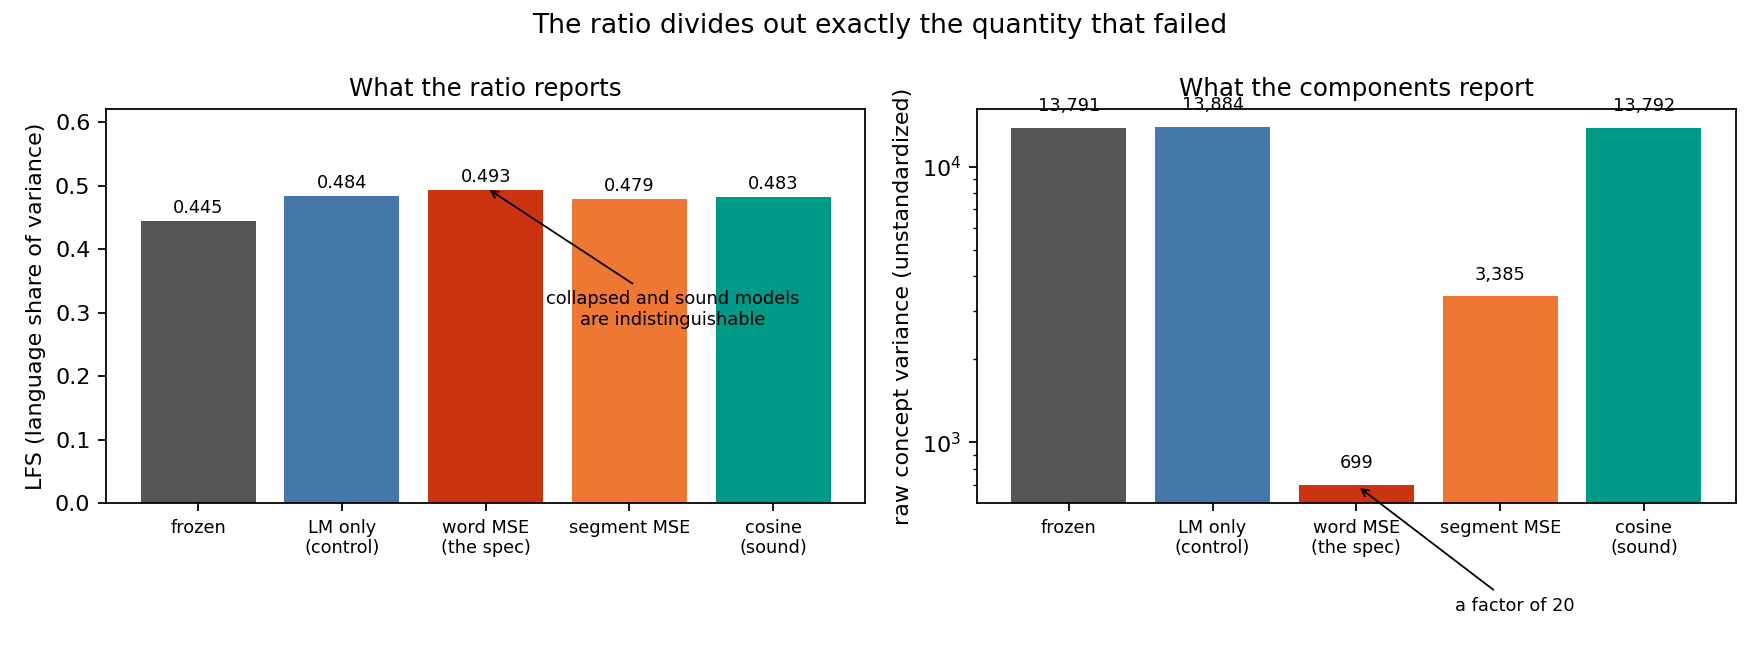
\includegraphics[width=0.95\linewidth]{figs/report/fig17_ratio_hides_scale.png}
\caption{Report Figure 14 and paper appendix figure. The collapse condition read two ways.}\label{fig:g-r17}\end{figure}

\paragraph{Report Figure 14 (ratio against components).} Five training conditions
of Qwen3-0.6B on the word-alignment objectives. Left: LFS for each condition, all
between $0.445$ and $0.493$. Right, logarithmic axis: raw concept variance at
the same layer, $13{,}791$ for the frozen model and $699$ for the word-MSE
condition. What to look for: the condition that lost 95 percent of its concept variance
is indistinguishable from the sound conditions on the left and stands out by a
factor of twenty on the right. Sentence: ``The ratio divides out the quantity
that failed; report the components.'' This is the single most important
figure for the ``why not a score'' argument.

\begin{figure}[h]\centering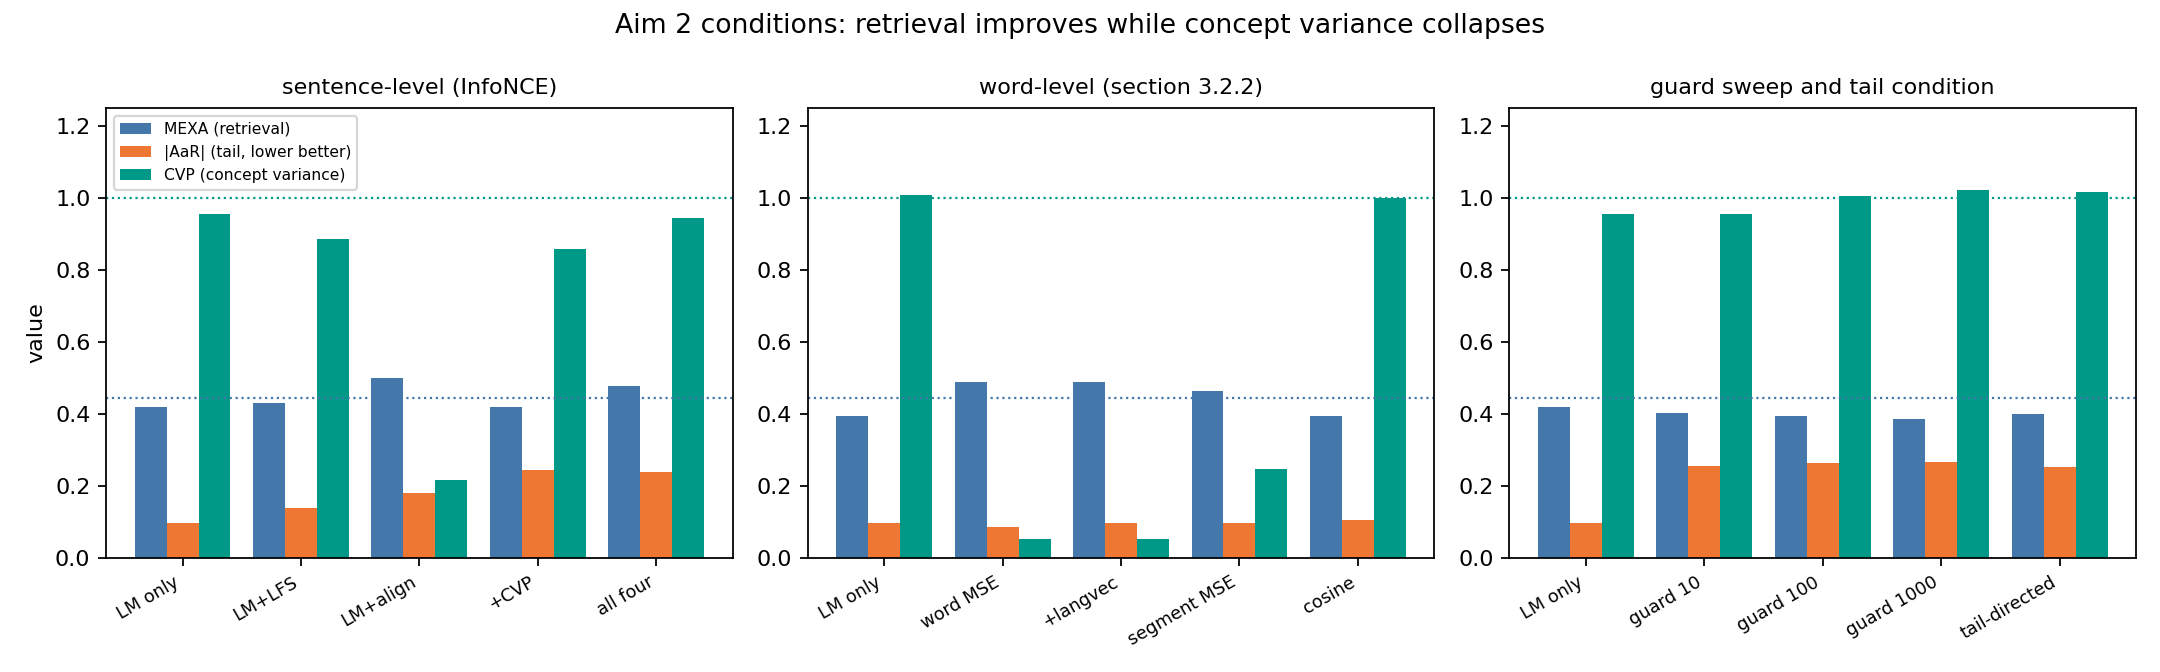
\includegraphics[width=0.95\linewidth]{figs/report/fig18_aim2_arms.png}
\caption{Report Figure 15. Every Aim 2 condition on three instruments.}\label{fig:g-r18}\end{figure}

\paragraph{Report Figure 15 (Aim 2 conditions).} Three panels for three objective
families; within each, one group of three bars per condition: MEXA (retrieval),
the magnitude of AaR (tail, lower is better), and CVP, concept-variance
preservation relative to the frozen model. Dotted lines mark the frozen
model's retrieval and CVP of 1. What to look for: in the word-level panel,
retrieval rises for the word-MSE and language-vector conditions while their CVP
falls to about $0.05$; the cosine condition keeps CVP at 1 and gains nothing.
Sentence: ``Objectives that improve alignment scores can do so by shrinking
the representation; only the preservation measure catches it.''

\begin{figure}[h]\centering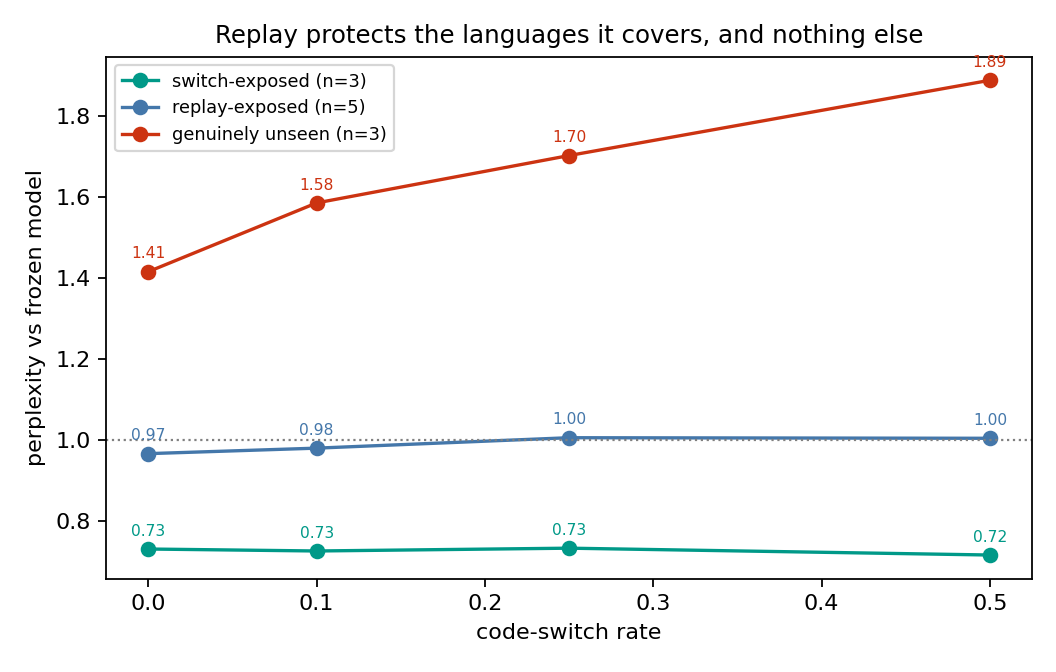
\includegraphics[width=0.66\linewidth]{figs/report/fig20_codeswitch_cost.png}
\caption{Report Figure 16. Code-switched training cost by language group.}\label{fig:g-r20}\end{figure}

\paragraph{Report Figure 16.} Horizontal axis: the code-switch rate used in
training. Vertical axis: perplexity relative to the frozen model, so 1.0 is
unchanged and higher is worse. Three groups of languages: those present in
the switched data, those protected by replay, and those genuinely unseen.
What to look for: the unseen group degrades monotonically, to $1.89$ times
worse at a 50 percent rate, while the other two groups sit at or below 1.
Sentence: ``Replay protects what it contains and nothing else.''

\begin{figure}[h]\centering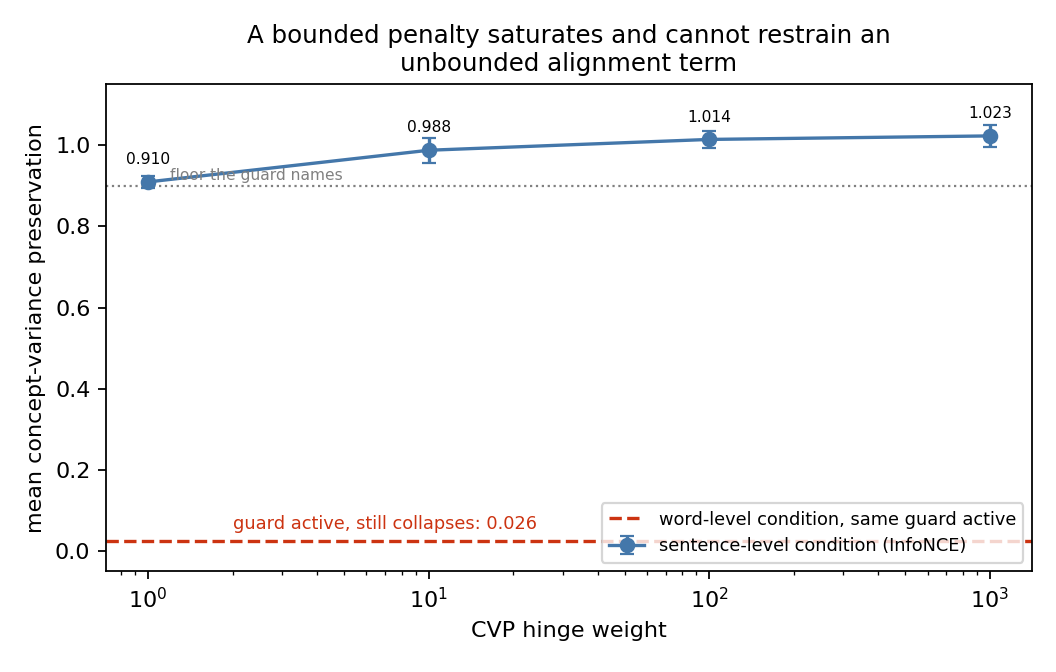
\includegraphics[width=0.66\linewidth]{figs/report/fig21_guard_sweep.png}
\caption{Report Figure 17. The concept-variance guard sweep.}\label{fig:g-r21}\end{figure}

\paragraph{Report Figure 17.} Horizontal axis, logarithmic: the weight on
the concept-variance hinge penalty, from 1 to 1000. Vertical axis: mean
concept-variance preservation. The blue curve is the sentence-level
contrastive condition, rising from $0.91$ to $1.02$ and flattening. The dashed red
line at $0.026$ is the word-level condition with the same guard active. Sentence:
``A bounded penalty saturates; it cannot restrain an unbounded alignment
term, so the guard has to be a constraint, not a weight.''

\begin{figure}[h]\centering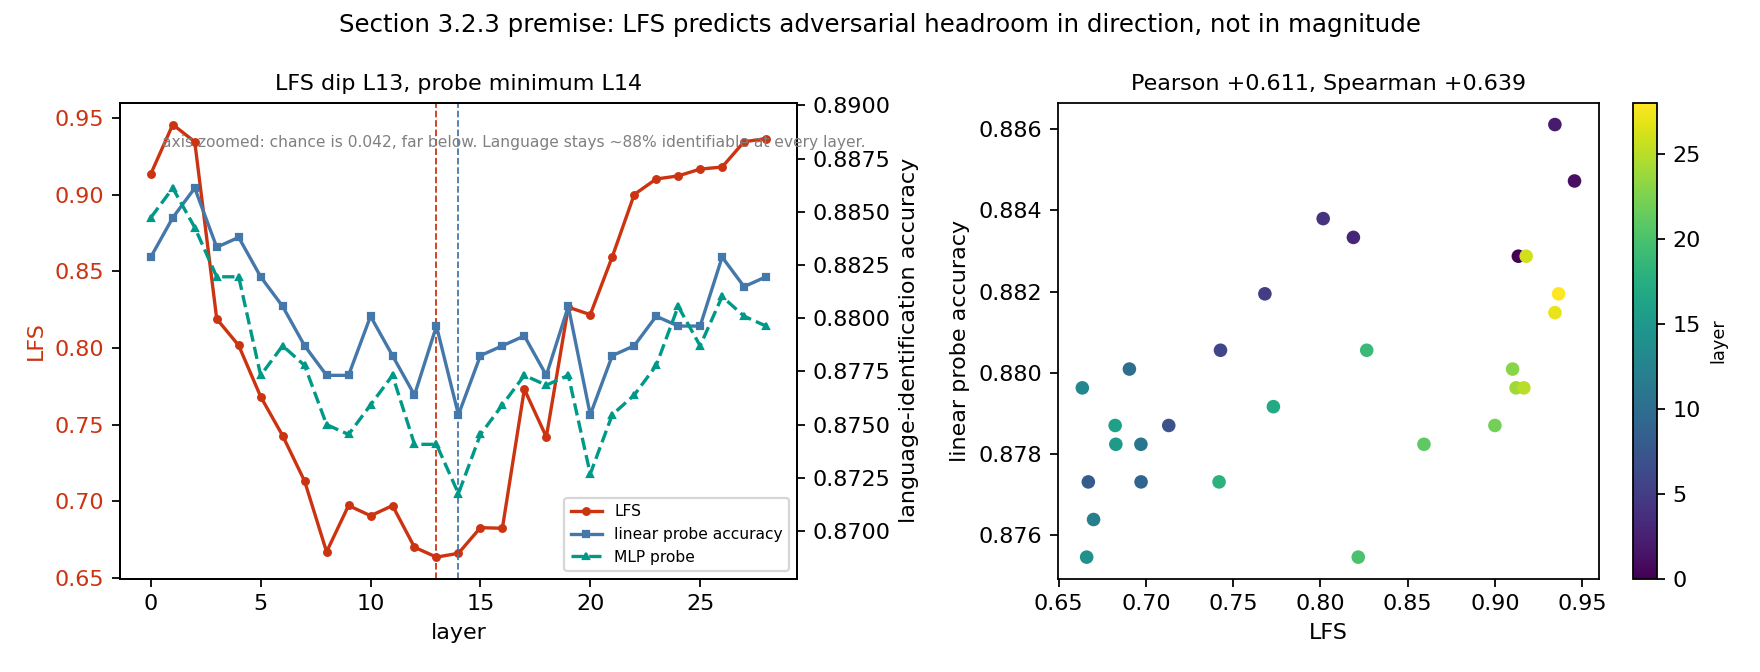
\includegraphics[width=0.95\linewidth]{figs/report/fig19_adversarial_probe.png}
\caption{Report Figure 18. LFS against language-identification probe accuracy.}\label{fig:g-r19}\end{figure}

\paragraph{Report Figure 18 (probe).} Left: layers of Qwen3-0.6B on the
horizontal axis; LFS in red on the left axis; accuracy of a classifier that
predicts the language from the hidden state in blue (linear) and green
(small network) on the right axis. Read the right axis carefully: it runs
from $0.870$ to $0.890$, a zoom; chance is $0.042$. Dashed verticals mark the
LFS minimum at layer 13 and the probe minimum at layer 14. Right: the same
29 layers as a scatter, LFS against probe accuracy, Pearson $0.61$. What to
look for: the curves move together in direction, but the probe never drops
below 87 percent. Sentence: ``Even at the dip, the language is almost
perfectly readable from the representation; the dip is about the share of
variance, not about erasing language identity.'' This is why ``lower LFS''
must never be read as ``language-agnostic''.

\subsection{Figure-measure habits worth keeping}

\begin{itemize}[leftmargin=1.2em]
\item Find the null or the chance line before judging any level. LFS has
$0.298$ on this grid; the benchmark has $0.25$.
\item A depth axis is relative unless it says ``layer''; the same relative
depth is a different layer in a 25-layer and a 49-layer model.
\item Two vertical axes (report Figures 3a and 11) invite a false measure of
the crossing point. Read each curve against its own axis.
\item A ratio next to a raw component (report Figure 14) is the habit the
paper asks the field to adopt.
\item Every number in a figure traces to an artifact in the claims ledger;
if a reviewer asks where a bar came from, the answer is a file path and a job
identifier.
\end{itemize}
